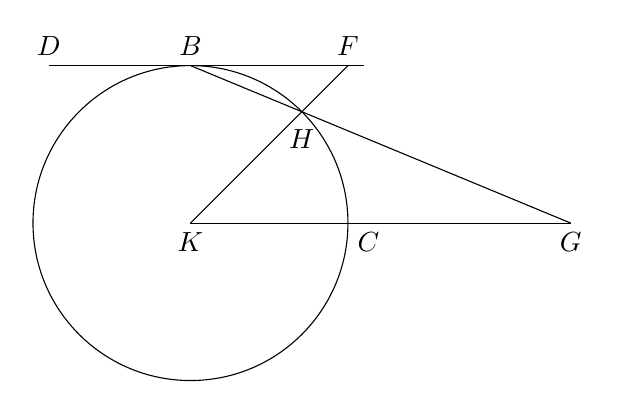
\begin{tikzpicture}
	\draw (0,0) circle (2);
	\draw (0,0) node[below]{$K$} -- ({2+2*sqrt(2)},0) node[below]{$G$};
	\draw (-1.8,2) node[above]{$D$} -- (2.2,2);
%	\draw (0,2) -- (4,0);
	\draw (0,0) -- (2,2) node[above]{$F$};
	\draw (0,2) node[above]{$B$} -- ({2+2*sqrt(2)},0);
	\node[below right] at (2,0) {$C$};
	\node[below, outer sep=3] at ({sqrt(2)},{sqrt(2)}) {$H$};
\end{tikzpicture}